\documentclass[12pt,a4paper]{article}
\usepackage[italian]{babel}
\usepackage[utf8]{inputenc}
\usepackage{fourier} 

% Images
\usepackage{graphicx}
\usepackage{caption}
\usepackage{subcaption}
\graphicspath{ {../Images} }

\begin{document}

\title{\textbf{Tour guidato per bambini ai musei civici}}
\author{Alice Balestieri}
\date{}

\maketitle
\newpage

\section{Che cosa spiegare:}

	\begin{enumerate}
		
	\item Mostrare la \textbf{Pala Bellini}. Evidenziando il dettaglio della \textit{Colomba} che rappresenta lo \textit{Spirito Santo}, presente nel pannello centrale contenente la scena dell'Incoronazione della Vergine e il dettaglio del \textit{Drago di S. Giorgio}, presente in basso tra i sette riquadri della predella.
	% Add images here
	\item Mostrare quadri che fanno uso della prospettiva, confrontandoli con quelli che ne sono privi.  
	\item Spiegare gli elementi che contraddistinguono la \textbf{Collezione Rossini}; come il \textit{Rosso vermiglio} e \textit{l'oro ed i gioielli} nei dipinti.
	\begin{figure}[h]
		\centering
		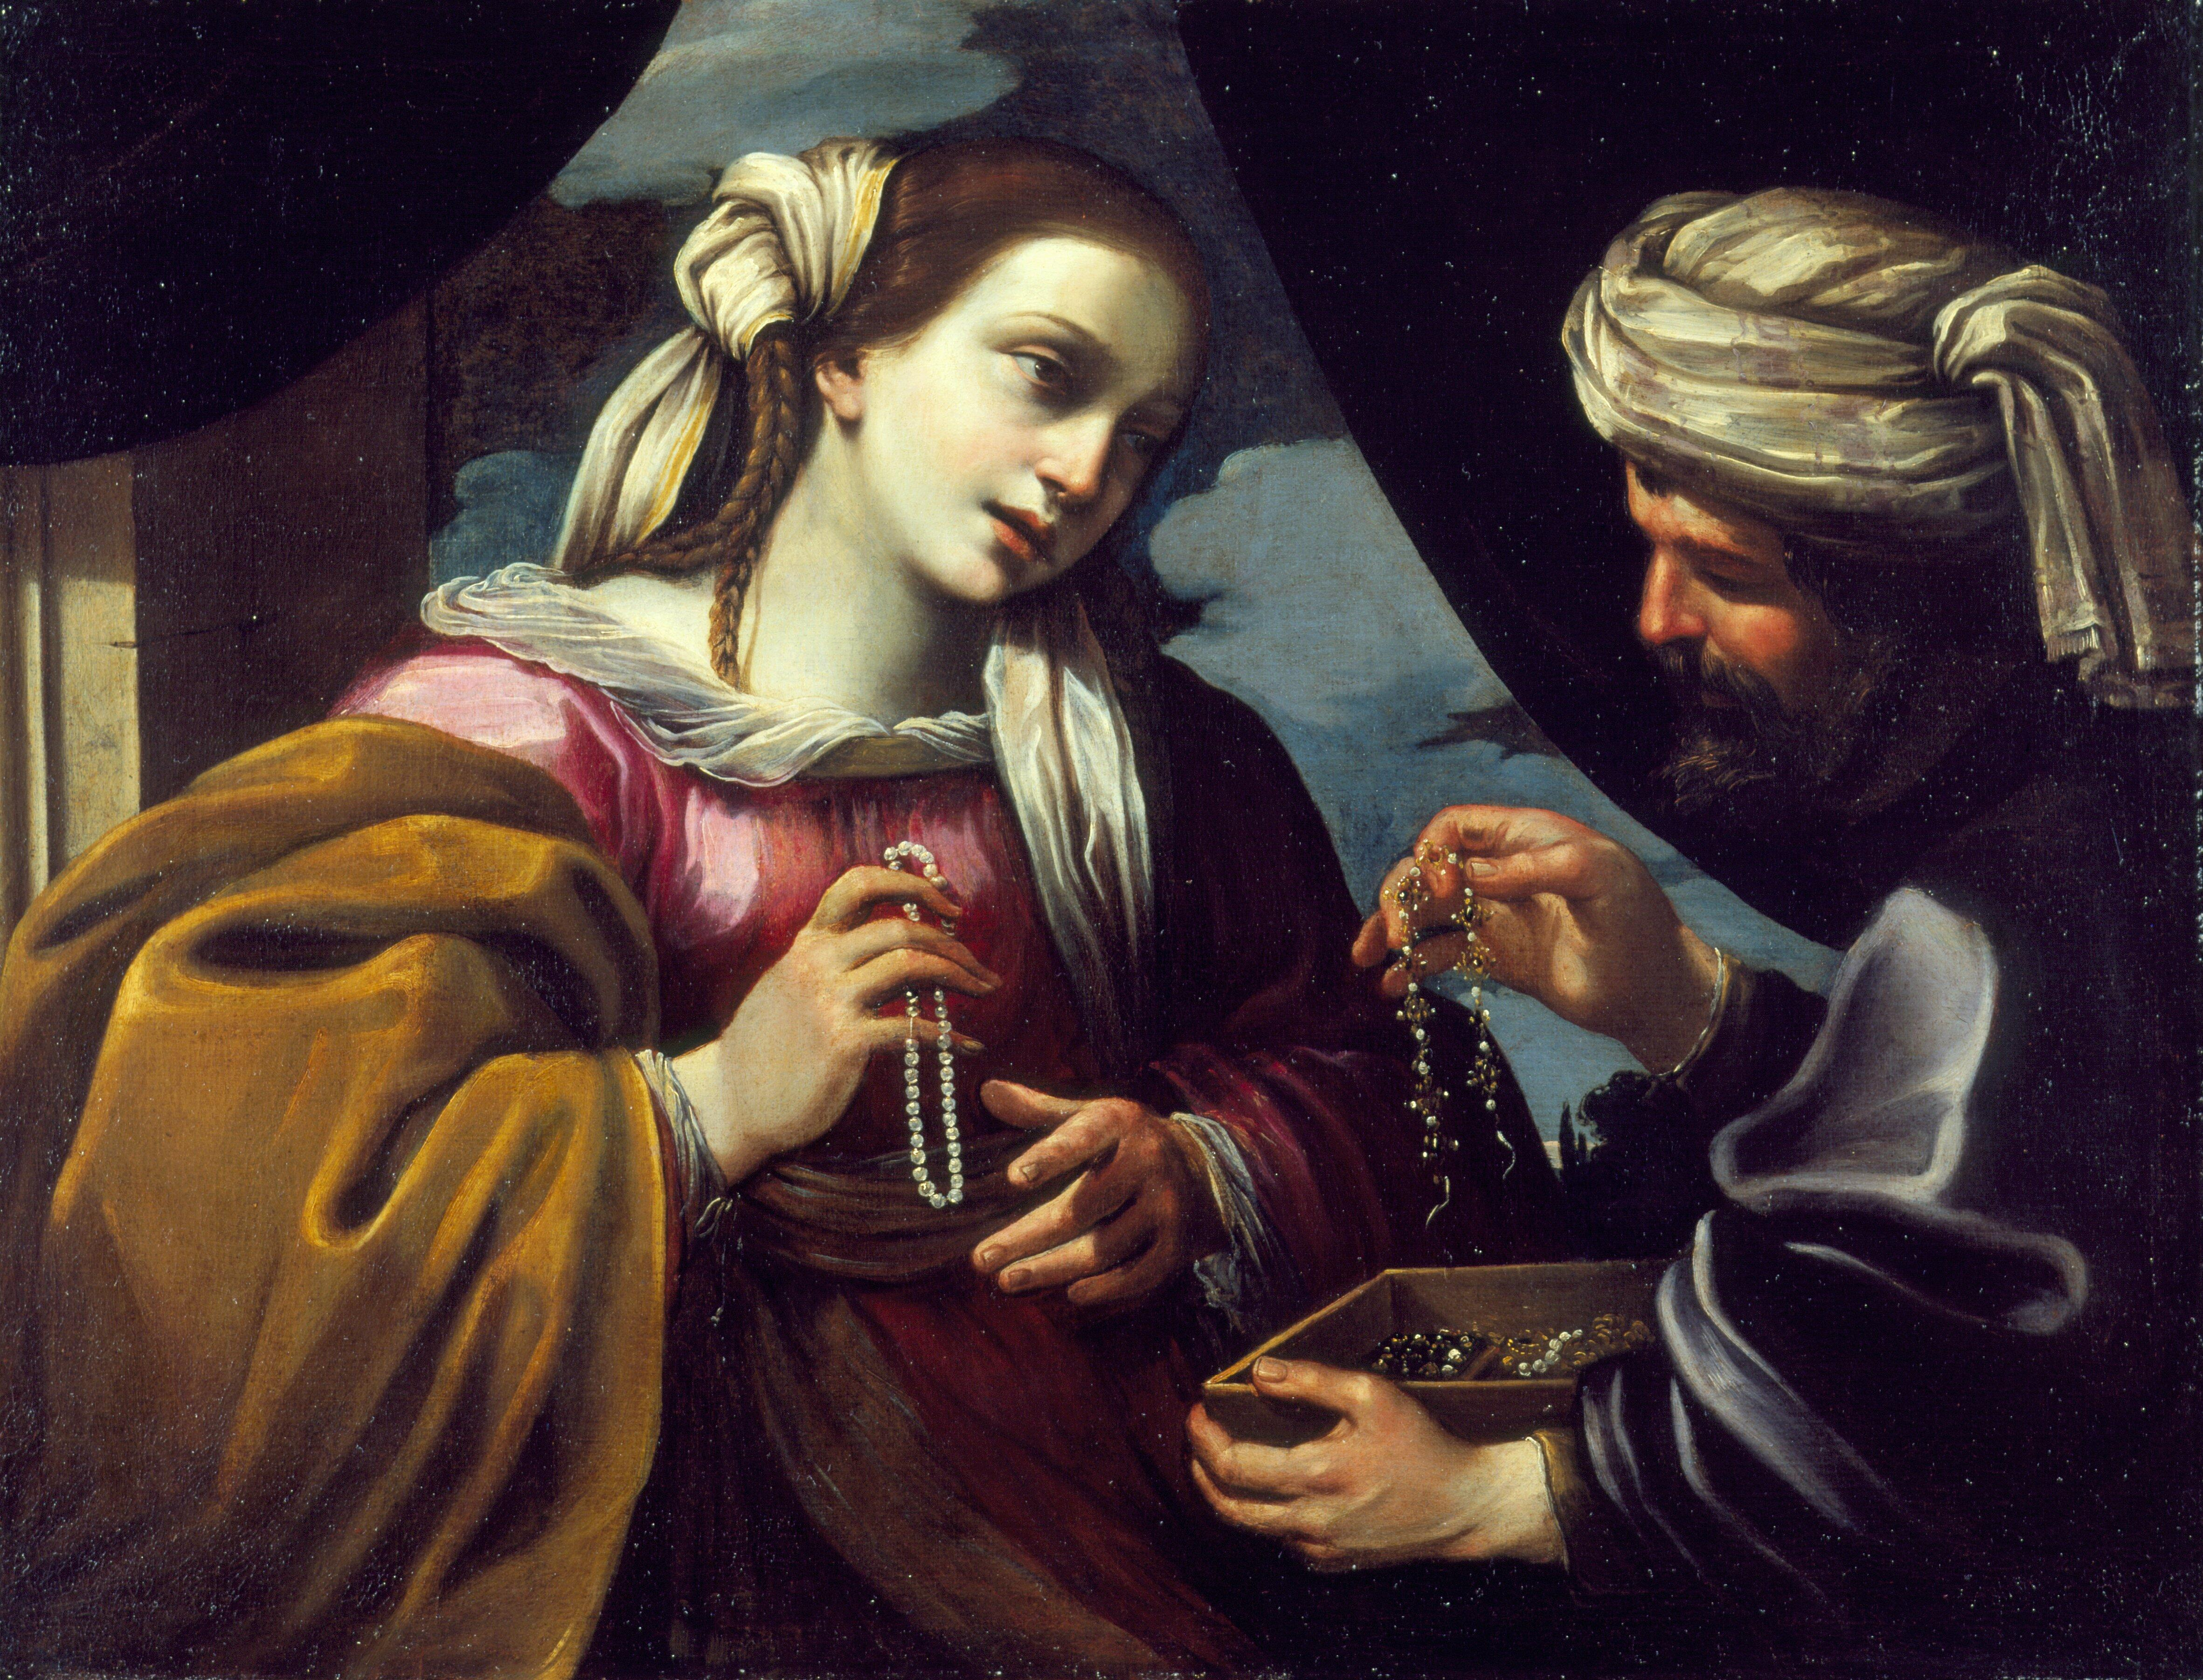
\includegraphics[scale = 0.05]{Pietro_Desani_Rebeca_y_Eleazar.jpg}
		\caption{Pietro Desani - Rebeca y Eleazar.}
	\end{figure}
	
	\item Mostrare la \textbf{ceramica della collezione Mazza} dove è presente lo \textit{scoiattolo nero di cinquecento anni fa}.
	% Add image here
	\item Esporre in maniera semplice: lo \textbf{specchio in vetro di Murano} decorato con \textit{incisioni d'uva d'argento},  gli \textbf{oggetti in avorio e madreperla}, lo \textbf{Stipo con vedute di Roma} facendo riferimento alle \textit{cartoline} di Pesaro e l'\textbf{Orologio Notturno}.
	% Add images here
	\item Mostrare il \textbf{Piatto della bottega pesarese} con \textit{decoro della rosa di Pesaro}.
	\begin{figure}[h]
		\centering
		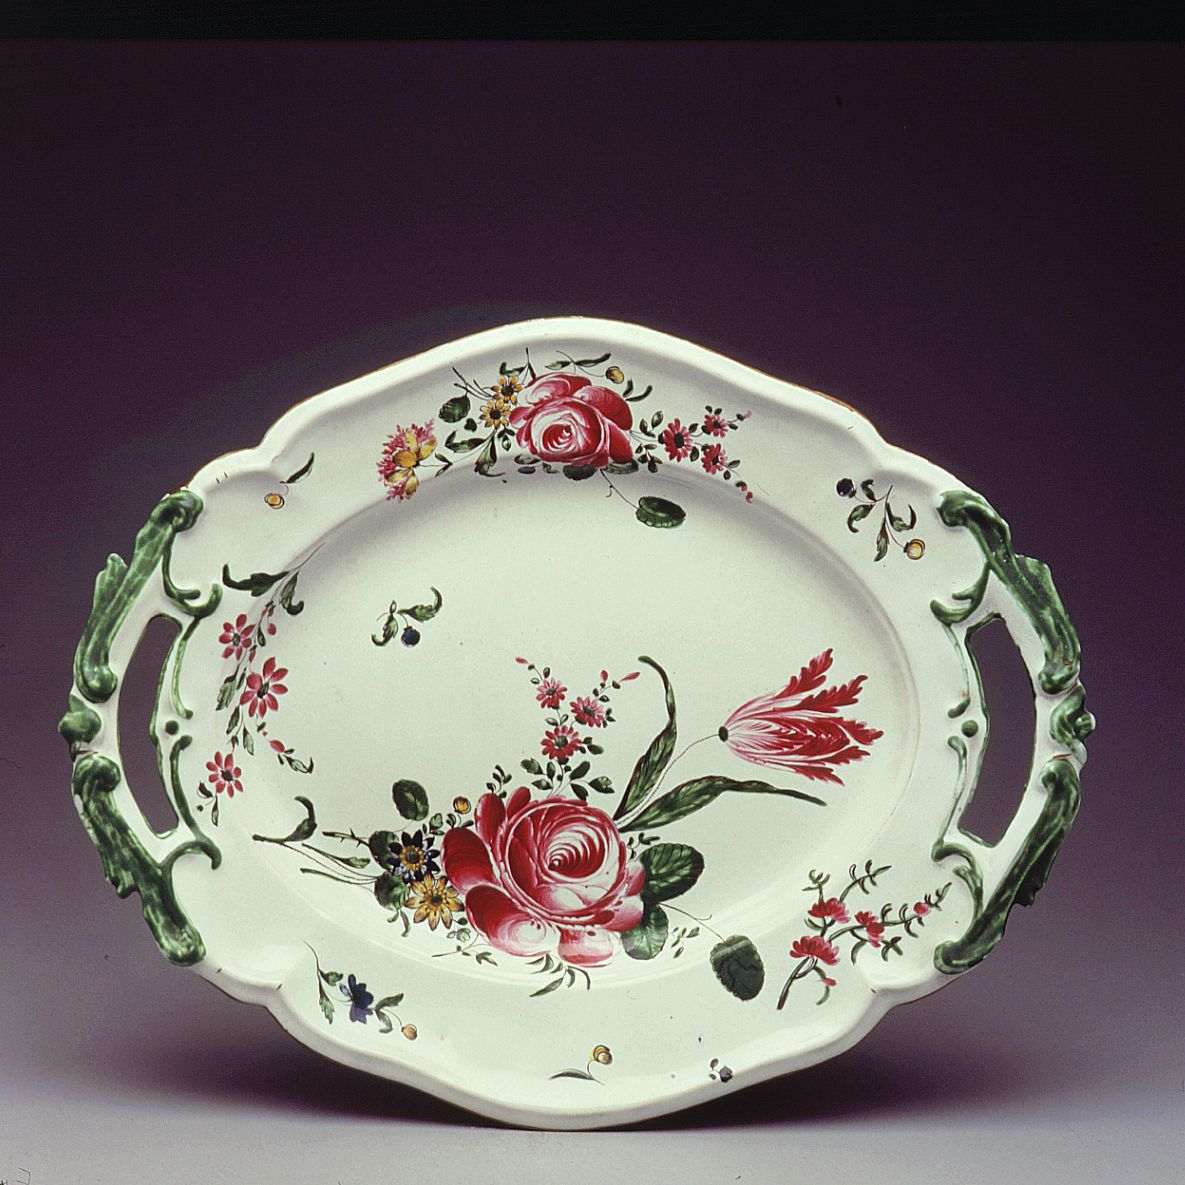
\includegraphics[]{Piatto_pesaro.jpg}
		\caption{Piatto - bottega pesarese.}
	\end{figure}
	
	\item Mostrare le \textbf{Nature Morte}, evidenziando la \textit{frutta} ed i \textit{calici in vetro}, mostrare il \textbf{Trompe l'oeil} con il \textit{Sonetto di Antonio Gianlisi Junior} e il \textbf{Trompe l'oeil} con la \textit{pipa} mettendo in risalto i cibi e gli oggetti di uso comune come la \textit{pipa} e i \textit{savoiardi} che alludono ai Savoia.
	%Add images here
	\item Mostrare dipinti contenenti particolari che possono attirare l'attenzione dei bambini, come per esempio \textit{le uova, i salami ed i limoni} nel dipinto \textbf{Dispensa con dolci, uova, salame, formaggi, ghiacciata e canestro di limoni} oppure il dettaglio del \textit{cinghiale} presente nella \textbf{Morte di Adone}.
	\begin{figure}[h]
		\centering
		\begin{subfigure} [h]{0.4\textwidth}
			\centering
			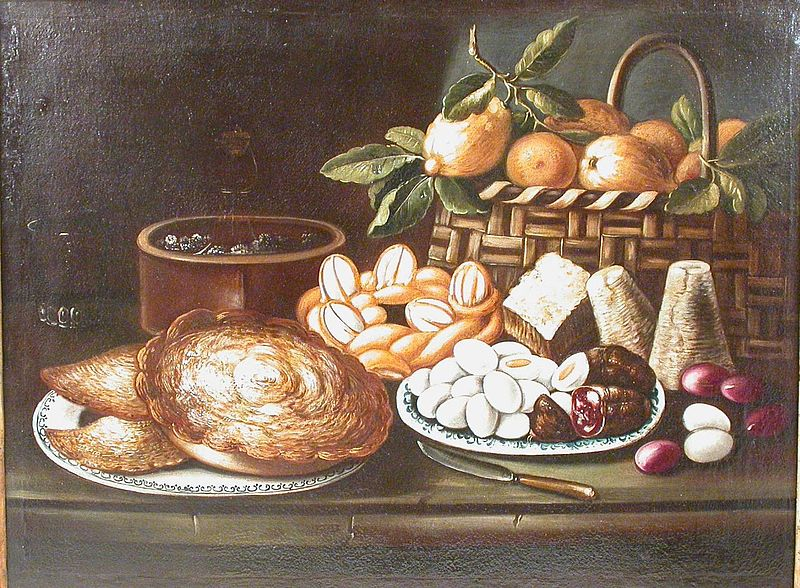
\includegraphics[]{Dispensa_natura_morta.jpg}
			\caption{Tommaso Realfonso - Dispensa con dolci, uova, salame, formaggi, ghiacciaia e canestro di limoni.}
		\end{subfigure}
	\hfill
		\begin{subfigure}[h] {0.4\textwidth}
			\centering
			\includegraphics[scale=0.3]{Morte_di_Adone.jpg}
			\caption{Francesco Gessi - Morte di Adone.}
		\end{subfigure}
	\end{figure}
	
	\end{enumerate}
\newpage
\listoffigures

\end{document}